\documentclass[11pt, english]{article}
\usepackage[english]{babel}
\usepackage[utf8]{inputenc}

\usepackage{geometry}
\geometry{
	a4paper,
	left=20mm,
	top=30mm,
	right=20mm
}

\usepackage{listings}
\usepackage{amsmath}
\usepackage{amsfonts}
\usepackage{amssymb}
\usepackage{amsthm} 
\usepackage{mathrsfs}
\usepackage{mathabx}
\usepackage{graphicx}
\usepackage{eurosym}
\usepackage{subfigure}
\usepackage{dsfont}
\usepackage{bbm}
%\lstdefinestyle{myCustomMatlabStyle}{
%	language=Matlab,
%	numbers=left,
%	stepnumber=1,
%	numbersep=10pt,
%	tabsize=4,
%	showspaces=false,
%	showstringspaces=false
%}

\usepackage{graphicx} 
\usepackage{fancyvrb} 
\usepackage{listings} 
\usepackage{listings}
\usepackage{amsmath}
\usepackage{amsfonts}
\usepackage{amssymb}
\usepackage{amsthm} 
\usepackage{mathrsfs}
\usepackage{mathabx}
\usepackage{graphicx}
\usepackage{eurosym}
\usepackage{subfigure}
\usepackage{dsfont}
\usepackage{bbm}
\usepackage{inputenc}

% Default fixed font does not support bold face
\DeclareFixedFont{\ttb}{T1}{txtt}{bx}{n}{12} % for bold
\DeclareFixedFont{\ttm}{T1}{txtt}{m}{n}{12}  % for normal

% Custom colors
\usepackage{color}
\definecolor{deepblue}{rgb}{0,0,0.5}
\definecolor{deepred}{rgb}{0.6,0,0}
\definecolor{deepgreen}{rgb}{0,0.5,0}

\newcommand\pythonstyle{\lstset{
		language=Python,
		%basicstyle=\ttm,
		otherkeywords={self},             % Add keywords here
		keywordstyle=\ttb\color{deepblue},
		emph={MyClass,__init__},          % Custom highlighting
		emphstyle=\ttb\color{deepred},    % Custom highlighting style
		stringstyle=\color{deepgreen},
		frame=tb,                         % Any extra options here
		showstringspaces=false            % 
		breaklines=true,% automatic line breaking
		basicstyle=\small,% basic font style 
		numbers=left,% display line numbers on the left side 
		numberstyle=\scriptsize,% use small line numbers 
		numbersep=10pt,% space between line numbers and code 
		tabsize=3,% sizes of tabs 
		showstringspaces=false,% do not replace spaces in strings by a certain character 
		captionpos=b,% positioning of the caption below 
		breaklines=true,% automatic line breaking 
}}


% Python environment
\lstnewenvironment{python}[1][]
{
	\pythonstyle
	\lstset{#1}
}
{}

% Python for external files
\newcommand\pythonexternal[2][]{{
		\pythonstyle
		\lstinputlisting[#1]{#2}}}

% Python for inline
\newcommand\pythoninline[1]{{\pythonstyle\lstinline!#1!}}


\lstdefinestyle{myCustomMatlabStyle2}{% setup listings 
	language=R,% set programming language 
	basicstyle=\small,% basic font style 
	keywordstyle=\bfseries,% keyword style 
	commentstyle=\ttfamily\itshape,% comment style 
	numbers=left,% display line numbers on the left side 
	numberstyle=\scriptsize,% use small line numbers 
	numbersep=10pt,% space between line numbers and code 
	tabsize=3,% sizes of tabs 
	showstringspaces=false,% do not replace spaces in strings by a certain character 
	captionpos=b,% positioning of the caption below 
	breaklines=true,% automatic line breaking 
	escapeinside={(*}{*)},% escaping to LaTeX 
	fancyvrb=true,% verbatim code is typset by listings 
	extendedchars=false,% prohibit extended chars (chars of codes 128--255) 
	literate={"}{{\texttt{"}}}1{<-}{{$\leftarrow$}}1{<<-}{{$\twoheadleftarrow$}}1 
	{~}{{$\sim$}}1{<=}{{$\le$}}1{>=}{{$\ge$}}1{!=}{{$\neq$}}1{^}{{$^\wedge$}}1,% item to replace, text, length of chars 
	alsoletter={.<-},% becomes a letter 
	alsoother={$},% becomes other 
	otherkeywords={!=, ~, $, *, \&, \%/\%, \%*\%, \%\%, <-, <<-, /},% other keywords 
	deletekeywords={c}% remove keywords 
}

\newcommand{\grafico}[5]{
	\begin{figure}
		[h!tbp]
		\centering
		\includegraphics[scale=#2, angle=#3]{#1}
		%\captionsetup{width=13cm}
		\caption{#4\label{#5}}
	\end{figure}
}

\newcommand{\su}[2]{\sum\limits_{#1}^{#2}}

\setlength{\parindent}{0pt}
\begin{document}
\title{Stochastic Models and Optimization: Problem Set 4}
\author{Roger Garriga Calleja, José Fernando Moreno Gutiérrez, David Rosenfeld, Katrina Walker}
\date{\today}
\maketitle
\section*{Q1}

We are given a linear-quadratic problem with perfect state information but with a forecast. We first set up the primitives of the system:\\
$x_k$: the state in period k\\
$u_k$: the decision variable in period k\\
$w_k$: the disturbances in period k\\
$y_k$: an accurate prediction that $w_k$ will be selected according to a particular probability distribution $P_{k|y_k}$\\
\\
We set up the dynamics of the problem with a linear system, as follows:
$$x_{k+1} = A_kx_k + B_ku_k + w_k$$
Where A and B are $n \times n$ matrices.\\
We also have a quadratic cost:
$$g_N(x_N) = x_N'Q_Nx_N$$
$$g_k(x_k) = x_k'Q_kx_k + u_k'R_ku_k$$
Where $Q_k$ and $R_k$ are $n \times n$ positive definite matrices.\\
\\
Our problem is thus to minimise:
$$E[\sum_{k=0}^{N-1}(x_k'Q_kx_k + u_k'R_ku_k) + x_N'Q_Nx_N]$$
Subject to:
$$x_{k+1} = A_kx_k + B_ku_k + w_k$$
\\
We can now set up our DP-algorithm:
$$J_N(x_N, y_N) = x_N'Q_Nx_N$$
$$J_k(x_k, y_k) = \min_{u_k \in R^n}E_{w_k}[x_k'Q_kx_k + u_k'R_ku_k + J_{k+1}(x_{k+1}, y_{k+1})]$$
\\
We can see that $J_N(x_N)$ is of the form $J(x_k, y_k) = x_k'K_kx_k + x_k'b_k(y_k) + c(y_k)$, with$Q_n = K_n$, $x_N'b_N(y_N) = 0$ and $c(y_k) = 0$.\\
We assume that this is also true at stage k+1, so that:
$$J(x_{k+1}, y_{k+1}) = x_{k+1}'K_{k+1}x_{k+1} + x_{k+1}'b_{k+1}(y_{k+1}) + c(y_{k+1})$$
Where $b_{k+1}(y_{k+1})$ is an n-dimensional vector and $c(y_{k+1})$ is a scalar.
Using this, we can compute $J_k(x_k, y_k)$:
\begin{align*}
	J_k(x_k, y_k) &=  \min_{u_k \in R^n}E_{w_k}[x_k'Q_kx_k + u_k'R_ku_k + J_{k+1}(x_{k+1}, y_{k+1})]=\\
	& = \min_{u_k \in R^n}E_{w_k}[x_k'Q_kx_k + u_k'R_ku_k + x_{k+1}'K_{k+1}x_{k+1} + x_{k+1}'b_{k+1}(y_{k+1}) + c(y_{k+1})\\
	&= \min_{u_k \in R^n}E_{w_k}[x_k'Q_kx_k + u_k'R_ku_k + (A_kx_k + B_ku_k + w_k)'K_{k+1}(A_kx_k + B_ku_k + w_k) +\\
	&+ (A_kx_k + B_ku_k + w_k)'b_{k+1}(y_{k+1}) + c(y_{k+1})]= x_k'(Q_k + A_k'K_{k+1}A_k)x_k + E[w_k'K_{k+1}w_k] +\\
	&+ \min_{u_k \in R^n}[u_k'(R_k + B_k'K_{k+1}B_k)u_k + 2x_k'A_kK_{k+1}B_ku_k + 2u_kB_kK_{k+1}E[w_k|y_k] +\\
	&+ u_k'B_k'b_{k+1}(y_{k+1})] + x_k'A_k'K_{k+1}E[w_k|y_k] + x_k'A_k'b_{k+1}(y_{k+1}) + E[w_k|y_k]'b_{k+1}(y_{k+1})
\end{align*}


We then find our optimal decision by taking the derivative of $J_k(x_k, y_k)$ with respect to $u_k$ and set it equal to zero in order to solve for our optimal solution $u*$:
$$2(R_k + B_k'K_{k+1}B_k)u_k^* + 2B_k'K_{k+1}A_kx_k + 2B_kK_{k+1}B_k + 2B_kK_{k+1}E[w_k|y_k] + B_k'b_{k+1}(y_{k+1}) = 0$$
$$u_k^* = (R_k + B_k'K_{k+1}B_k)^{-1}B_k'K_{k+1}(A_kx_k + E[w_k|y_k]) + \alpha_k$$
Where $\alpha_k = B_k'b_{k+1}(y_{k+1})$
\newpage
\section*{Q2}

(ii)\\
\begin{center}
	\begin{figure}[h]\small
		\centering
		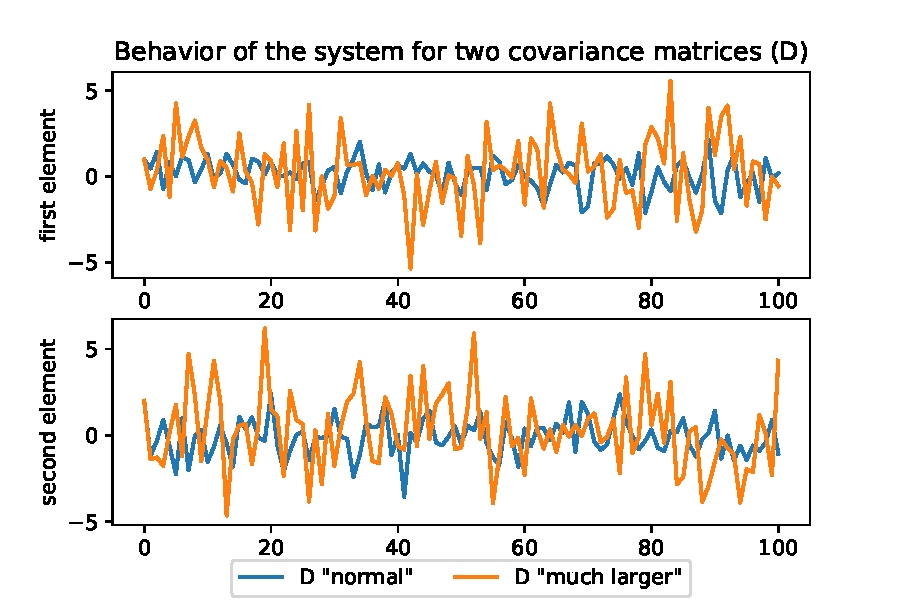
\includegraphics[height=8cm,width=10cm, page=1]{figures}
	\end{figure}
\end{center}

\textbf{Python Code:}\\

\pythonexternal{code.py}
\newpage
\section*{Q3}
\textbf{Asset selling w/offer estimation}\\
\\
\underline{Primitives}\\
\begin{itemize}
\item $x_k$ current offer.
\item  $\{w_k\}$ iid offers with an unknown underlying distribution $F_1$ or $F_2$.
\item constraints: selling ($u_1$) or not selling ($u_2$)):
$\left \{\begin{tabular}{lll}
	\{$u^1, u^2$\} \ \textup{if} \ $x_k$ $\neq$ T\\
	0,  otherwise
\end{tabular} \right.\\ 
$\item rewards:
$g_n(x_N) =$
$\left \{
\begin{tabular}{lll}
 $x_N$, \textup{if} \ $x_N$ $\neq$ T\\
0,  otherwise
\end{tabular}\right.\\
g_k(x_k, u_k, w_k)$ = 
$ \left \{ 
\begin{tabular}{lll}
$(1 + r)^{N-k}x_k$, \textup{if} \ $x_k$ $\neq$ T and if $u_k$ = $u^1$\\
	0,  otherwise 
\end{tabular}
\right.$
\item $q$ = prior belief that $F_1$ is true 
\item $q_{k+1} = \frac{\mathds{P}\{y_k = y^1|w_0,\dots,w_{k}\}}{\mathds{P}(w_1 = w_1)}$
= $\frac{q_kF_1(w_k)}{q_kF_1(w_k) + (1-q)F_2(w_k)}$
\end{itemize}
Now, we can apply the DP algorithm to find an optimal asset selling policy\\ \\
$J_{N-1}(x_{N-1}) = $
$ \left \{ 
\begin{tabular}{lll}
$\max\{(1 + r)x_k,(q_{N-1}\mathds{E}_{F_1}[J_N(w_{N-1})] + (1-q_{N-1})\mathds{E}_{F_2}[J_{N}(w_{N-1})])$ if $x_{N-1}\neq T$\\
0,  otherwise 
\end{tabular}\\
\right.$
\\\\
$ J_k(x_k) = $
$ \left\{
\begin{tabular}{lll}
$\textup{max}(q_{k}\mathds{E}_{F_1}[J_{k+1}(w_{k})] + (1-q_{k})\mathds{E}_{F_2}[J_{k+1}(w_{k})]),(1 + r)^{N-k}x_k$ if $x_k\neq T$\\
	0,  otherwise 
\end{tabular}
\right.$\\\\
Thus, the threshold for selling an asset will be:
$(1 + r)^{N-k}x_k\geq q_{k}\mathds{E}_{F_1}[J_{k+1}(w_{k})] + (1-q_{k})\mathds{E}_{F_2}[J_{k+1}(w_{k})]$ \\\\
So, the optimal asset selling policy will be:
$\mu^*(x_k) =$
$ \left \{
\begin{tabular}{lll}
$u^1, x_{k+1}\geq \frac{q_{k}\mathds{E}_{F_1}[J_{k+1}(w_{k})] + (1-q_{k})\mathds{E}_{F_2}[J_{k+1}(w_{k})]}{(1 + r)^{N-k}}$\\
$u^2$, otherwise
\end{tabular}
\right.$
\newpage
\section*{Q4}

This problem is basically the same as the inventory management considering the demand as a random variable following an unknown distribution. It is a case with imperfect state information, in which the distribution of demand will be either $F_1$ or $F_2$. The probability that the demand follows $F_1$ is updated at each period $k$ after observing the realization of the demand. That will effect the way the expectation of the demand is computed.\\

\underline{Primitives:\\}

$x_k$: items in the inventory at period $k$.\\
$u_k$: quantity ordered at period $k$.\\
$w_k$: demand during period $k$. $w_k$ are iid with probability distribution either $F_1$ or $F_2$.\\
$q_k$: probability that $w_k$ follows distribution $F_1$.\\
$q_0=q$: a priori probability that demand follows the distribution $F_1$.\\

\underline{Dynamics:\\}

$x_{k+1}=x_k+u_k-w_k$\\
$q_{k+1}=\frac{q_kf_1(w_k)}{q_kf_1(w_k)+(1-q_k)f_2(w_k)}$, where $f_i(w)$ is the pdf of the distribution $F_i$.\\

\underline{Cost:\\}

$g_N(x_N)=0$.\\
$g_k(x_k,u_k,w_k)=cu_k+h\max\{0,w_k-x_k-u_k\}+p\max\{0,x_k+u_k-w_k\}$, where $c,h,p$ are positive and $p>c$.\\

\underline{DP algorithm:}\\

$J_N(x_N)=0$\\
$J_k(x_k)=\underset{u_k\geq 0}{\min}\mathbb{E}\left[cu_k+h\max\{0,w_k-x_k-u_k\}+p\max\{0,x_k+u_k-w_k\}+J_{k+1}(x_{k+1})\right]$\\

In order to solve it we can introduce the variable $y_k=x_k+u_k$, and the we have \\
$J_k(y_k)=\underset{u_k\geq x_k}{\min}G_k(y_k)-cx_k$, where $$G_k(y_k)=cy+h\mathbb{E}[\max\{0,w_k-y_k\}]+p\mathbb{E}[\max\{0,y_k-w_k\}]+\mathbb{E}[J_{k+1}(y_k-w_k)].$$
Now, since $w_k$ is drawn from $F_1$ with probability $q_k$ and from $F_2$ with probability $F_2$ we can apply the law of total probabilities, leading to\\
\begin{align*}
G(y_k)=cy_k+q_k(h\mathbb{E}_{w_k|w\sim F_1}[\max\{0,w_k-y_k\}]+p\mathbb{E}_{w_k|w\sim F_1}[\max\{0,y_k-w_k\}]+\mathbb{E}_{w_k|w\sim F_1}[J_{k+1}(y_k-w_k)])+\\
+(1-q_k)(h\mathbb{E}_{w_k|w\sim F_2}[\max\{0,w_k-y_k\}]+p\mathbb{E}_{w_k|w\sim F_2}[\max\{0,y_k-w_k\}]+\mathbb{E}_{w_k|w\sim F_2}[J_{k+1}(y_k-w_k)]).
\end{align*}
We saw in class that $cy_k+h\mathbb{E}_{w_k|w\sim F_i}[\max\{0,w_k-y_k\}]+p\mathbb{E}_{w_k|w\sim F_i}[\max\{0,y_k-w_k\}]+\mathbb{E}_{w_k|w\sim F_i}[J_{k+1}(y_k-w_k)]$ is convex, since we have a sum of convex, our $G(y_k)$ will also be convex. So, there exists a $S_k$ that will represent the optimal stock we seek at period $k$. However, $S_k$ could be smaller than $x_k$, so it would not be reachable (in which case we would not by stock). Then, the policy will be
\begin{equation*}
\mu_k^*(x_k)=\left\{\begin{array}{ll}
S_k-x_k & \text{if } S_k>x_k\\
0 & \text{otherwise.}
\end{array}\right.
\end{equation*}  
\newpage
\section*{Q5}

(a) To find the policy that will minimize the cost function in the worst case. We can write a DP-like algorithm to solve this problem as\\
$J_N(x_N)=g_N(x_N)$\\
$J_k(x_k)=\underset{\mu_k\in U_k}{\min\ }\underset{w_k\in W_k(x_k,\mu_k(x_k))}{\max\ }[g_k(x_k,\mu_k(x_k),w_k)+J_{k+1}(x_{k+1})]$, where $x_{k+1}=f_k(x_k,\mu_k(x_k),w_k)$ $\forall k=0,\dots, N-1$.\\

(b) In this problem the state $x_k$ needs to belong to a certain set $X_k$ at each state $k$, so we have to choose a policy that will assure that this will happen. We write the dynamics in a general form like \\
$x_{k+1}=f(x_k,\mu_k(x_k))+h_k(w_k)$.\\
We consider a cost of the policy $g(\mu_k(x_k))$ and the cost of being outside $X_k$ infinite to ensure we stay whenever possible there.\\

\underline{DP algorithm:}\\

$J_N(x_N)=\left\{\begin{array}{ll}
0 & \text{if }x_N\in X_N\\
\infty & \text{otherwise}
\end{array}\right.$\\
$J_{k+1}=\underset{\mu_k(x_k)\in U_k}{\min\ }\underset{w_k\in W_k(x_k,\mu_k(x_k))}{\max\ }\left\{\begin{array}{ll}
g_k(\mu(x_k))+J_{k+1}(x_{k+1}) & \text{if } x_k\in X_k\\
\infty & \text{otherwise}
\end{array}\right.$,\\\\ where $x_{k+1}=f_k(x_k,\mu_k(x_k))+h_k(w_k)$. Then, we will need to compute recursively the $\bar{X}_k$ that allow to continue in the sets $X_{k+1},\dots,X_N$. In order to do so, $x_k$ will need to be in a certain set $Y_{k+1}$ such that for any $w_k\in W_k$, $f(x_k,\mu_k(x_k))+h(w_k)$ belong to $\bar{X}_{k+1}$. Initializing $\bar{X}_N=X_N$, $\forall k=1,\dots,N-1$, the recursion would be the next:\\

$Y_{k+1}=\{z\in \mathcal{X}: z+h_k(w_k)\in\bar{X}_{k+1},\forall w_k\in W_k(x_k,\mu_k(x_k))\}$\\

$\bar{X}_k=\{x\in X_k: \exists \mu_k(x)\in U_k\text{ such that }  f_k(x,\mu_k(x_k))\in Y_{k+1}\}$




\end{document}
